% ========================================
%	Header einbinden
% ========================================

\documentclass[bibtotoc,titlepage]{scrartcl}

% Deutsche Spracheinstellungen
\usepackage[ngerman,german]{babel, varioref}
\usepackage[T1]{fontenc}
\usepackage[utf8]{inputenc}

%\usepackage{marvosym}

\usepackage{amsfonts}
\usepackage{amssymb}
\usepackage{amsmath}
\usepackage{amscd}
\usepackage{amstext}
\usepackage{float}
\usepackage{caption}
\usepackage{wrapfig}
\usepackage{setspace}
\usepackage{threeparttable}
\usepackage{footnote}

\newfloat{formel}{htbp}{for}
\floatname{formel}{Formel}


\usepackage{longtable}

%\usepackage{bibgerm}

\usepackage{footnpag}

\usepackage{ifthen}                 %%% package for conditionals in TeX
\usepackage[amssymb]{SIunits}
%Fr textumflossene Bilder und Tablellen
%\usepackage{floatflt} - veraltet

%Fr Testzwecke aktivieren, zeigt labels und refs im Text an.
%\usepackage{showkeys}

% Abstand zwischen zwei Abs�zen nach DIN (1,5 Zeilen)
% \setlength{\parskip}{1.5ex plus0.5ex minus0.5ex}

% Einrckung am Anfang eines neuen Absatzes nach DIN (keine)
%\setlength{\parindent}{0pt}

% R�der definieren
% \setlength{\oddsidemargin}{0.3cm}
% \setlength{\textwidth}{15.6cm}

% bessere Bildunterschriften
%\usepackage[center]{caption2}


% Probleml�ungen beim Umgang mit Gleitumgebungen
\usepackage{float}

% Nummeriert bis zur Strukturstufe 3 (also <section>, <subsection> und <subsubsection>)
%\setcounter{secnumdepth}{3}

% Fhrt das Inhaltsverzeichnis bis zur Strukturstufe 3
%\setcounter{tocdepth}{3}

\usepackage{exscale}

\newenvironment{dsm} {\begin{displaymath}} {\end{displaymath}}
\newenvironment{vars} {\begin{center}\scriptsize} {\normalsize \end{center}}


\newcommand {\en} {\varepsilon_0}               % Epsilon-Null aus der Elektrodynamik
\newcommand {\lap} {\; \mathbf{\Delta}}         % Laplace-Operator
\newcommand {\R} { \mathbb{R} }                 % Menge der reellen Zahlen
\newcommand {\e} { \ \mathbf{e} }               % Eulersche Zahl
\renewcommand {\i} { \mathbf{i} }               % komplexe Zahl i
\newcommand {\N} { \mathbb{N} }                 % Menge der nat. Zahlen
\newcommand {\C} { \mathbb{C} }                 % Menge der kompl. Zahlen
\newcommand {\Z} { \mathbb{Z} }                 % Menge der kompl. Zahlen
\newcommand {\limi}[1]{\lim_{#1 \rightarrow \infty}} % Limes unendlich
\newcommand {\sumi}[1]{\sum_{#1=0}^\infty}
\newcommand {\rot} {\; \mathrm{rot} \,}         % Rotation
\newcommand {\grad} {\; \mathrm{grad} \,}       % Gradient
\newcommand {\dive} {\; \mathrm{div} \,}        % Divergenz
\newcommand {\dx} {\; \mathrm{d} }              % Differential d
\newcommand {\cotanh} {\; \mathrm{cotanh} \,}   %Cotangenshyperbolicus
\newcommand {\asinh} {\; \mathrm{areasinh} \,}  %Area-Sinus-Hyp.
\newcommand {\acosh} {\; \mathrm{areacosh} \,}  %Area-Cosinus-H.
\newcommand {\atanh} {\; \mathrm{areatanh} \,}  %Area Tangens-H.
\newcommand {\acoth} {\; \mathrm{areacoth} \,}  % Area-cotangens
\newcommand {\Sp} {\; \mathrm{Sp} \,}
\newcommand {\mbe} {\stackrel{\text{!}}{=}}     %Must Be Equal
\newcommand{\qed} { \hfill $\square$\\}
\renewcommand{\i} {\imath}
\def\captionsngerman{\def\figurename{\textbf{Abb.}}}

%%%%%%%%%%%%%%%%%%%%%%%%%%%%%%%%%%%%%%%%%%%%%%%%%%%%%%%%%%%%%%%%%%%%%%%%%%%%
% SWITCH FOR PDFLATEX or LATEX
%%%%%%%%%%%%%%%%%%%%%%%%%%%%%%%%%%%%%%%%%%%%%%%%%%%%%%%%%%%%%%%%%%%%%%%%%%%%
%%%
\ifx\pdfoutput\undefined %%%%%%%%%%%%%%%%%%%%%%%%%%%%%%%%%%%%%%%%% LATEX %%%
%%%
\usepackage[dvips]{graphicx}       %%% graphics for dvips
\DeclareGraphicsExtensions{.eps,.ps}   %%% standard extension for included graphics
\usepackage[ps2pdf]{thumbpdf}      %%% thumbnails for ps2pdf
\usepackage[ps2pdf,                %%% hyper-references for ps2pdf
bookmarks=true,%                   %%% generate bookmarks ...
bookmarksnumbered=true,%           %%% ... with numbers
hypertexnames=false,%              %%% needed for correct links to figures !!!
breaklinks=true,%                  %%% breaks lines, but links are very small
linkbordercolor={0 0 1},%          %%% blue frames around links
pdfborder={0 0 112.0}]{hyperref}%  %%% border-width of frames
%                                      will be multiplied with 0.009 by ps2pdf
%
\hypersetup{ pdfauthor   = {Hannes Franke; Julius Tilly},
pdftitle    = {V301 Innenwiderstand und Leistungsanpassung}, pdfsubject  = {Protokoll FP}, pdfkeywords = {V301, Innenwiderstand, Leistungsanpassung},
pdfcreator  = {LaTeX with hyperref package}, pdfproducer = {dvips
+ ps2pdf} }
%%%
\else %%%%%%%%%%%%%%%%%%%%%%%%%%%%%%%%%%%%%%%%%%%%%%%%%%%%%%%%%% PDFLATEX %%%
%%%
\usepackage[pdftex]{graphicx}      %%% graphics for pdfLaTeX
\DeclareGraphicsExtensions{.pdf}   %%% standard extension for included graphics
\usepackage[pdftex]{thumbpdf}      %%% thumbnails for pdflatex
\usepackage[pdftex,                %%% hyper-references for pdflatex
bookmarks=true,%                   %%% generate bookmarks ...
bookmarksnumbered=true,%           %%% ... with numbers
hypertexnames=false,%              %%% needed for correct links to figures !!!
breaklinks=true,%                  %%% break links if exceeding a single line
linkbordercolor={0 0 1},
linktocpage]{hyperref} %%% blue frames around links
%                                  %%% pdfborder={0 0 1} is the default
\hypersetup{
pdftitle    = {V301 Innenwiderstand und Leistungsanpassung}, 
pdfsubject  = {Protokoll AP}, 
pdfkeywords = {V301, Innenwiderstand, Leistungsanpassung},
pdfsubject  = {Protokoll AP},
pdfkeywords = {V301, Innenwiderstand, Leistungsanpassung}}
%                                  %%% pdfcreator, pdfproducer,
%                                      and CreationDate are automatically set
%                                      by pdflatex !!!
\pdfadjustspacing=1                %%% force LaTeX-like character spacing
\usepackage{epstopdf}
%
\fi %%%%%%%%%%%%%%%%%%%%%%%%%%%%%%%%%%%%%%%%%%%%%%%%%%% END OF CONDITION %%%
%%%%%%%%%%%%%%%%%%%%%%%%%%%%%%%%%%%%%%%%%%%%%%%%%%%%%%%%%%%%%%%%%%%%%%%%%%%%
% seitliche Tabellen und Abbildungen
%\usepackage{rotating}
\usepackage{ae}
\usepackage{
  array,
  booktabs,
  dcolumn
}
\makeatletter 
  \renewenvironment{figure}[1][] {% 
    \ifthenelse{\equal{#1}{}}{% 
      \@float{figure} 
    }{% 
      \@float{figure}[#1]% 
    }% 
    \centering 
  }{% 
    \end@float 
  } 
  \makeatother 


  \makeatletter 
  \renewenvironment{table}[1][] {% 
    \ifthenelse{\equal{#1}{}}{% 
      \@float{table} 
    }{% 
      \@float{table}[#1]% 
    }% 
    \centering 
  }{% 
    \end@float 
  } 
  \makeatother 
%\usepackage{listings}
%\lstloadlanguages{[Visual]Basic}
%\allowdisplaybreaks[1]
%\usepackage{hycap}
%\usepackage{fancyunits}

% ========================================
%	Angaben für das Titelblatt
% ========================================

\title{Versuch 21 - Optisches Pumpen\\				% Titel des Versuchs 
\large TU Dortmund, Fakultät Physik\\ 
\normalsize Fortgeschrittenen-Praktikum}

\author{Jan Adam\\			% Name Praktikumspartner A
{\small \href{jan.adam@tu-dortmund.de}{jan.adam@tu-dortmund.de}}	% Erzeugt interaktiven einen Link
\and						% um einen weiteren Author hinzuzfügen
Dimitrios Skodras\\					% Name Praktikumspartner B
{\small \href{dimitrios.skodras@tu-dortmund.de}{dimitrios.skodras@tu-dortmund.de}}		% Erzeugt interaktiven einen Link
}
\date{05. März 2014}				% Das Datum der Versuchsdurchführung

% ========================================
%	Das Dokument beginnt
% ========================================

\begin{document}

% ========================================
%	Titelblatt erzeugen
% ========================================

\maketitle					% Jetzt wird die Titelseite erzeugt
\thispagestyle{empty} 				% Weder Kopfzeile noch Fußzeile

% ========================================
%	Der Vorspann
% ========================================

%\newpage					% Wenn Verzeichnisse auf einer neuen Seite beginnen sollen
%\pagestyle{empty}				% Weder Kopf- noch Fußzeile für Verzeichnisse

\tableofcontents

%\newpage					% eine neue Seite
%\thispagestyle{empty}				% Weder Kopf- noch Fußzeile für Verzeichnisse
%\listoffigures					% Abbildungsverzeichnis

%\newpage					% eine neue Seite
%\thispagestyle{empty}				% Weder Kopf- noch Fußzeile für Verzeichnisse
%\listoftables					% Tabellenverzeichnis
\newpage					% eine neue Seite


% ========================================
%	Kapitel
% ========================================

%\section{Einleitung}				% Bei Bedarf

\section{Theorie}
\setcounter{page}{1}

\section{Durchführung}
\label{sec_durch}

\section{Auswertung}
\subsection{Vertikalkomponente des Erdmagnetfelds}
\begin{table}[H]
 \begin{tabular}{l|c|c|c}
  Spule & $r$ in cm & $N$ & $I/U$ in A/1\\
  \hline
  Vertikal & 11,735 & 20 & 1\\
  Horizontal & 15,790 & 154 & 0,1\\
  Sweep & 16,39 & 11 & 0,3
 \end{tabular}
\caption{Kenndaten benutzter Helmholtzspulen}
\label{tab_SpulenHor}
\end{table}
Um dem Einfluss des vertikalen Magnetfelds entgegenzuwirken, wird eine Helmholtz-Spule in die entsprechende Richtung orientiert, sodass das vom 
Stromfluss $I$ induzierte Magnetfeld $B$ genau dem des Erdmagnetfelds entspricht. $\mu_0$ ist die Vakuumpermeabilität, $r$ der Radius und $N$ die Windungszahl
Bei einer Umdrehungszahl von $U$=1,99 V und einem Widerstand von $R$ = 1 $\Omega$ wird kein Einfluss des vertikalen Erdmagnetfelds mehr festgestellt. 
Die Feldstärke $B_{\text{vert,Erde}}$ lässt nach Biot-Savart und mit Tabelle \ref{tab_SpulenHor} berechnen mit
\begin{equation}
 B_{\text{vert,Erde}} = \mu_0 \frac{8}{\sqrt{125}}\frac{I N}{r} = 30,5 \, \mu\text{T}.
\end{equation}
\subsection{Horizontalkomponente des Erdmagnetfelds}
Wie in \ref{sec_durch} beschrieben, wird die Resonanzfrequenz der RF-Spule stetig erhöht und ebenfalls das Magnetfeld der Horizontalspulen dahingehend,
dass die Transmission der Dampfzelle stark abnimmt. In Tabelle \ref{tab_SpulenHor} sind die Kenndaten der Horizontalspulen aufgeführt, die zur Umrechnung
der in den Tabellen \ref{tab_nuB1} und \ref{tab_nuB2} gelisteten Messwerte in Magnetfelder nötig sind.


\begin{minipage}{0.5\textwidth}
\begin{table}[H]
\begin{tabular}{c|cc|c}
$\nu$ in kHz & U$_{\text{sweep}}$ & U$_{\text{hor}}$ & $B_{r,1}$ in mT\\
\hline
 20 &	1,75&	0,00&	0,011\\
100&	3,70&	0,00&	0,022\\
200&	1,05&	0,12&	0,038\\
300&	1,55&	0,15&	0,049\\
400&	3,82&	0,15&	0,063\\
500&	2,48&	0,24&	0,078\\
600&	2,13&	0,30&	0,092\\
700&	2,27&	0,35&	0,106\\
800&	2,38&	0,40&	0,120\\
900&	2,60&	0,45&	0,134\\
1000&	2,73&	0,50&	0,148 \\
\end{tabular}
\caption{$\nu$ und $B_r$ des 1. Isotops}
\label{tab_nuB1}
\end{table}
\end{minipage}
\begin{minipage}{0,5\textwidth}
\begin{table}[H]
\begin{tabular}{c|cc|c}
$\nu$ in kHz & U$_{\text{sweep}}$ & U$_{\text{hor}}$ & $B_{r,2}$ in mT\\
\hline
20	&2,00&	0,00&	0,012\\
100&	4,90&	0,00&	0,030\\
200&	3,65&	0,12&	0,054\\
300&	5,11&	0,15&	0,070\\
400&	4,25&	0,25&	0,091\\
500&	2,74&	0,37&	0,114\\
600&	2,59&	0,45&	0,134\\
700&	1,78&	0,55&	0,155\\
800&	1,05&	0,65&	0,177\\
900&	2,47&	0,70&	0,199\\
1000&	1,55&	0,80&	0,220 \\
\end{tabular}
\caption{$\nu$ und $B_r$ des 2. Isotops}
\label{tab_nuB2}
\end{table}
\end{minipage}

Der Zusammenhang zwischen $\nu$ und $B_r$ wird zweimal mit einem linearen Ansatz
\begin{equation*}
 \nu = a\cdot B + b \hspace{2cm} \text{und} \hspace{2cm} \nu = c\cdot B + d
\end{equation*}
getestet und die Koeffizienten $a,b,c$ und $d$ durch GNUplot bestimmt. In Abbildung \ref{pic_nuB} sind die Messwerte dargestellt, sowie die eben
genannten linearen Ansätze als Fitgeraden.
\begin{figure}[h]
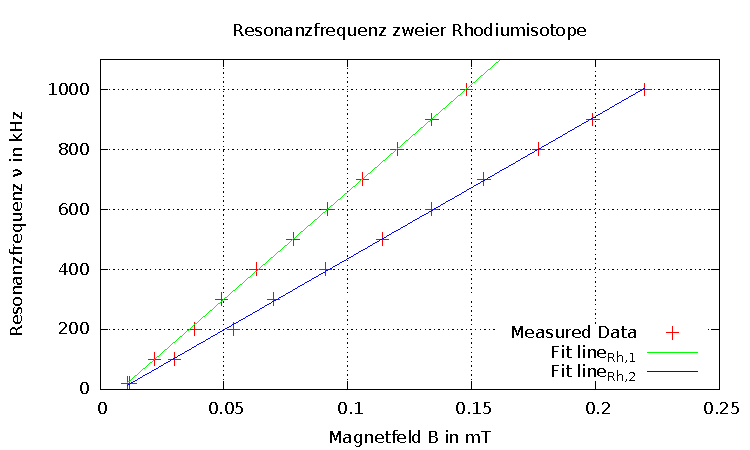
\includegraphics[width=0.8\textwidth]{../pics/v21B-nu.pdf}
\caption{Zusammenhang zwischen Resonanzfrequenz und Magnetfeld}
\label{pic_nuB}
\end{figure}
Hieraus ergeben sich die folgenden zwei Gleichungen
\begin{align}
 \nu_1 =& 7159(1\pm0,67\%)\frac{\text{kHz}}{\text{mT}}\cdot B - 58,6(1\pm6,1\%) \text{kHz}
 \label{eq_nu1}
 \end{align}
 \begin{align}
 \nu_2 =& 4741(1\pm0,70\%)\frac{\text{kHz}}{\text{mT}}\cdot B - 39,6(1\pm11,1\%) \text{kHz}.
 \label{eq_nu2}
\end{align}
Mit diesen zwei Gleichungen ist es nun möglich die Horizontalkomponente des Erdmagnetfelds zu ermitteln. Sie ist genau das Magnetfeld $B$, welches
die Gleichung \eqref{eq_nu1} bzw. \eqref{eq_nu2} 0 werden lässt. Aus den zwei Werten wird anschließend der Mittelwert genommen
\begin{align}
 B_1 = 8,19(1\pm6,1\%) \mu T \hspace{0.2cm} \text{und} \hspace{0.2cm} B_2 = 8,35(1\pm11,1\%) \mu T,
\end{align}
was schließlich zu einer Horizontalkomponente führt von
\begin{equation}
 B_{\text{hor}} = 8,27(1\pm12,7\% )\mu T.
\end{equation}
\subsection{Landé-Faktoren des Atoms}
\label{sec_lande}
Neben der Horizontalkomponente des Erdmagnetfelds kann man aus den Gleichungen \eqref{eq_nu1} und \eqref{eq_nu2} ebenfalls die Landé-Faktoren des
Atoms $g_F$ nach Gleichung \eqref{eq_nuB.g_F} errechnen, wo der Proportionalitätsfaktor mit $a$ bzw. $c$ identifiziert wird
\begin{equation}
 g_{F,1} = 0,511(1 \pm 0,67\%) \hspace{1cm}\text{und}\hspace{1cm}g_{F,2} = 0,339(1\pm 0,7\%) 
\end{equation}
Desweiteren lassen sich aus der Elektronenkonfiguration von Rubidium \cite{EKonf} die Drehimpulse bestimmen, sowie der Landé-Faktor der Elektronenhülle $g_J$.
Die Drehimpulse sind hierbei
\begin{equation}
 L = 0 , \qquad S=\frac12 , \qquad J = L+S = \frac12, \qquad F = I+J= I + \frac12,
\end{equation}
was nach \eqref{eq_gj} zu einem Faktor führt zu
\begin{equation}
 g_J = 2,0023. 
\end{equation}

\subsection{Kernspin $I$ der Rubidiumisotope}
Mit den Ergebnissen aus \ref{sec_lande} lassen sich nun nach \eqref{eq_gF(I)} die Kernspins der auftretenden Rubidiumisotope errechnen. Die etwas
längliche Formel ergibt umgestellt nach dem Kernspin
\begin{equation}
 I_k = \frac{1}{4\frac{g_{F,k}}{g_J}} \left[\left(1-4\frac{g_{F,k}}{g_J}\right) + \sqrt{\left(-1+4\frac{g_{F,k}}{g_J}\right)^2-12\frac{g_{F,k}}{g_J}\left(\frac{g_{F,k}}{g_J}-1\right)}\right]
\end{equation}
und führt zu
\begin{equation}
 I_1 = 1,459 \approx \frac32 \hspace{3cm} I_2=	2,459 \approx \frac52.
\end{equation}

\subsection{Isotopenverhältnis von $^{85}$Rb und $^{87}$Rb}
Durch das Auftauchen von zwei Resonanzfrequenzen bei denen die Transparenz der Probe einbricht, wird davon ausgegangen, dass es sich um zwei verschiedene
Isotope innerhalb der Probe handelt. Das Verhältnis ihres Vorkommens $N_i$ hängt mit dem Verhältnis der Transparenzaufhebung $A_i$ direkt zusammen
Die Bestimmung der Amplituden geschieht durch Ablesen am Oszilloskop in Abbildung \ref{pic_verh}
\begin{figure}[h]
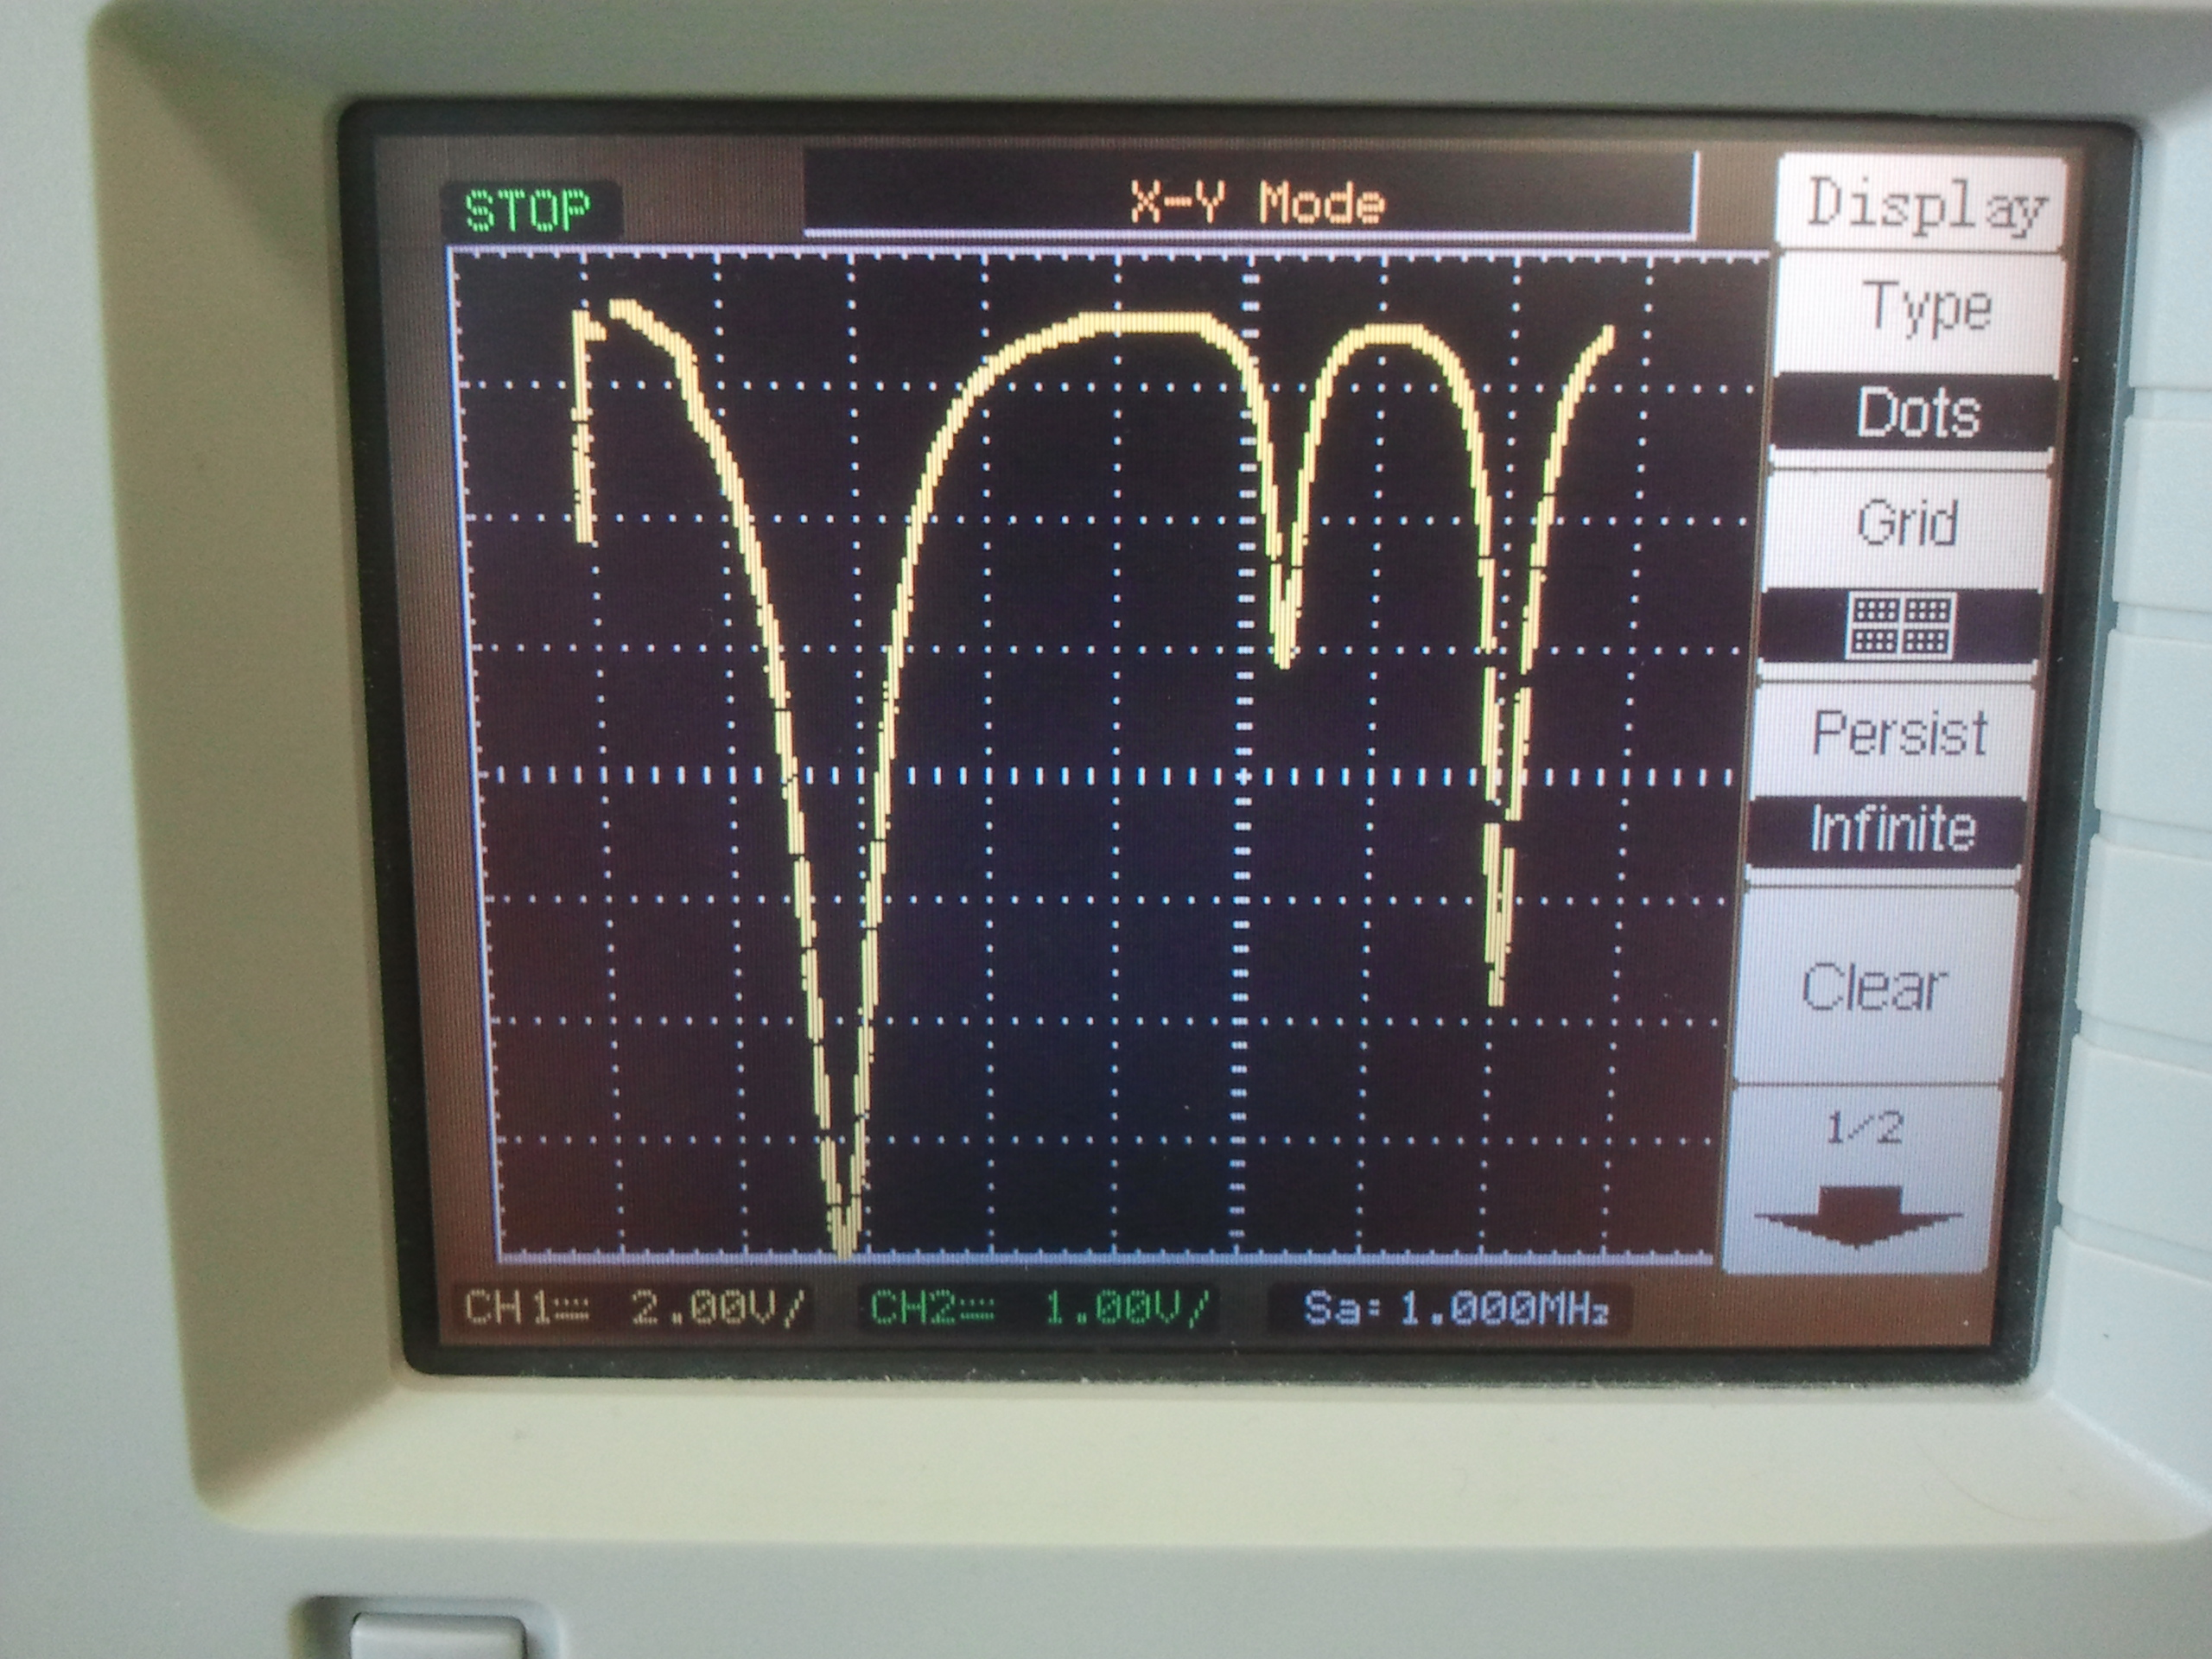
\includegraphics[width=0.8\textwidth]{../pics/v21Verh.jpg}
\caption{Typische Aufnahme am Oszilloskop, hier bei $\nu$ = 100 kHz}
\label{pic_verh}
\end{figure}\begin{equation}
 \frac{N_1}{N_2} = \frac{A_1}{A_2} = \frac{5,5}{2,5}= 2,2.
\end{equation}

\section{Diskussion}
\subsection{Erdmagnetfeld}
Die ermittelten Werte für die Vertikal- und Horizontalkomponente des Erdmagnetfelds sind anfolgend mit den Literaturwerten \cite{ErdB} verglichen. Die erheblichen
Fehler sind wohl auf ein ungenau Ausrichtung der Apparatur in Nord-Süd-Richtung zurückzuführen
\begin{equation}
 \frac{B_{\text{vert}}}{B_{\text{vert,Lit}}} = 70\% \hspace{3cm} \frac{B_{\text{hor}}}{B_{\text{hor,Lit}}} = 41\%
\end{equation}
\subsection{Eigenschaften von Rubidium}
Die erittelten Werte für die Landé-Faktoren $g_F$ haben zu den zwei Kernspins $I_1$ und $I_2$ geführt und werden anhand einer Nuklidkarte \cite{Spin} Rubidiumisotope
zugewiesen
\begin{equation}
 I_1 \approx \frac32 \rightarrow\, ^{87}\text{Rb} \hspace{2cm} I_2 \approx \frac52 \rightarrow\, ^{85}\text{Rb}.
\end{equation}
Das Verhältnis der Rb-Isotope \cite{Spin} wird mit dem Verhältnis der Amplituden verglichen, was zu folgender Übereinstimmung führt
\begin{equation}
 \frac{A_1}{A_2}\, /\, \frac{N_{^{85}\text{Rb}}}{N_{^{87}\text{Rb}}} = 2,2 \,/\, \frac{72,17\%}{27,83\%} =85\% .
\end{equation}



\begin{thebibliography}{xxxxxxxxxxx}
 \bibitem[PSE]{EKonf}Periodensystem der Elemente\\ \href{http://www.periodensystem.info/elemente/rubidium/}{periodensystem.info/elemente/rubidium/}
 \bibitem[Chemie.de]{ErdB}Form und Stärke des Erdmagnetfelds\\ \href{http://www.chemie.de/lexikon/Erdmagnetfeld.html#Form_und_St.C3.A4rke_des_Erdmagnetfeldes}{chemie.de/lexikon/Erdmagnetfeld}
 \bibitem[KAERI]{Spin}Nuklidkarte des \textit{Korea Atomic Energy Research Institute}\\ \href{http://atom.kaeri.re.kr/}{atom.kaeri.re.kr/}
\end{thebibliography}



\parskip 340pt
\Large{Literatur}\\\\

% ========================================
%	Literaturverzeichnis
% ========================================

%\bibliographystyle{plainnat}			% Bibliographie-Style auswählen
%\bibliography{BIBDATEI}			% Literaturverzeichnis

% ========================================
%	Das Dokument endent
% ========================================

\end{document}
